\documentclass{article}\twocolumn
\usepackage{./paper}

\graphicspath{ {../figures/} }

\title{Digital Camera Image Processing Pipeline Components}
\author{Hadleigh Nunes and Evan Lloyd New-Schmidt}
\date{Fall 2018}

\begin{document}

\maketitle


\begin{abstract}
    In this paper we explore concepts and methods for processing digital images in the initial stages of image development, including demosaicing, gamma correction, and white balance correction.
\end{abstract}

\section{Introduction}


% TODO: fig: overview of pipeline components

\begin{figure}[!h]
    \centering
    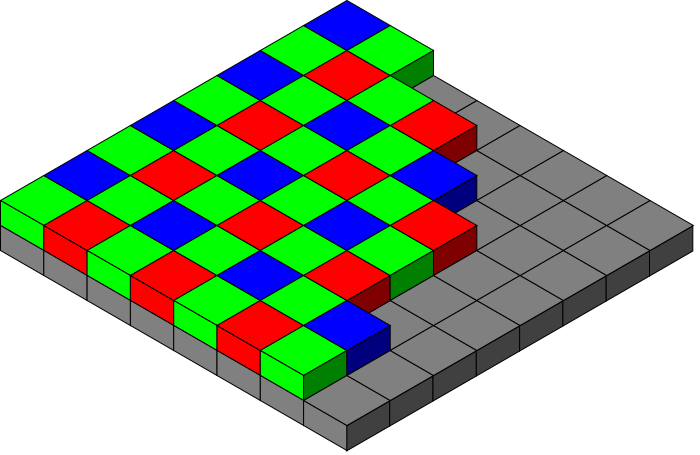
\includegraphics[width=\columnwidth]{bggr_bayer_pattern}
    \caption{Example of the BGGR Bayer grid used by the Raspberry Pi camera. Included from the \lstinline{picamera} module documentation\cite{picameradocs}.}
    \label{fig:my_label}
\end{figure}

% TODO: fig: bayer images comparison ala wikipedia

% TODO: fig: gamma curves
% TODO: fig: gamma correction image comparison

% TODO: fig: white balance comparison

\section{Mathematical Background}
The mathematical procedures we use are based mainly in Linear Algebra, Multivariable Calculus and Signal Processing. The simplest method of debayering is nearest neighbor interpolation, which we implemented by convolving a  $3x3$ kernel with each of the color channels. In the raw image, the matrix of each color channel contains values only in pixels corresponding to a sencel of the corresponding color. Pixel locations corresponding to a different color channel are occupied by zeros. By convolving the matrix 
    \begin{align}
        \threebythree{1}{1}{1}{1}{1}{1}{1}{1}{1}
    \end{align}
with each channel we are essentially averaging the adjacent pixel values of each pixel, including those diagonally adjacent. This is a rudimentary technique, and will create some artifacts, one of the more prominent being a 'zippering' effect caused by %TODO: details on zippering
There are many more complex approaches to debayering designed to reduce the artifacts created in the process. The first widely used such approach is the Kimmel algorithm, which models the image as a three dimensional surface, and interpolates in a direction orthogonal to the gradient, along the gentlest slope.

\section{Quantitative Procedure}

\subsection{Debayering}
    Out algorithm is based on a model of hue as a three dimensional surface. Similar to the Kimmel algorithm, we begin by interpolating missing values in the green channel, and then base the red and blue interpolations on the new green layer. 
    
    
    
\subsection{Gamma Correction}
    Raw digital images are often hard to interpret, as even when scaled to a full RGB range, the non-white parts of the image appear dark with little contrast. This effect occurs because the human eye perceives light non-linearly, meaning that though there may be a significant linear numerical variance in darker regions of an image, those differences are hard to interpret visually. To correct for this, the pixel values of a digital image are adjusted according to a power function. 
    \begin{equation}
        V_{out} = AV_{in}^{\gamma} \label{eqn:Gamma}
    \end{equation}
    The expression \eqref{eqn:Gamma} is the general form of the gamma function, where $A$ is a constant scalar, $V_{in}$ and $V_{out}$ are the input and output signals, respectively. 
    Typically for a "decoding" $\gamma$, a $\gamma$  function meant to re-scale a digital image for human viewing, a $\gamma < 1$ is used to enhance the visibility of non-white areas. 
\subsection{Sharpening}
    We use another convolution process to sharpen images. The kernel 
    \begin{align}
        \threebythree{0}{-1}{0}{-1}{5}{-1}{0}{-1}{0}
    \end{align}
    when convolved with an image produces a sharpened image, as color values which are highly present in neighboring pixels are reduced if not as present in the target pixel. This kernel works well for relatively low resolution images, but when applied to images with higher pixel density, the results are minimal. 

\subsection{Peak Signal-to-Noise Ratio (PSNR)}

Once we reconstruct the image using a demosaicing method, we compare it with the original image using Peak Signal-to-Noise Ratio (PSNR). This technique is used in several other papers to validate demosaicing techniques, including \cite{zapryanov_comparative_2008}, \cite{lukin_high-quality_2004}, and \cite{kimmel_demosaicing:_1999}.

%\subsection{White Balance}

\subsection{Further Applications}


\section{Results and discussion}

\section{Conclusion}


\section{Equations} 
\begin{equation}
    I^{R} = \rho _{R}(X)<\hat{\mathbf{N}}(x),\vec{l}>
    I^{G} = \rho _{G}(X)<\hat{\mathbf{N}}(x),\vec{l}>
\end{equation}
$\vec{l}$ is the light source direction, $\hat{\mathbf{N}}(x)$ is the normal vector to the surface at a pixel point

\begin{equation}
    \tilde{\mathbf{I}} = <\hat{\mathbf{N}}(x),\vec{l}>
\end{equation}

\begin{equation}
    \frac{\mathbf{I^{i}}}{\mathbf{I^{j}}} = \frac{\rho _{i}(X)\tilde{\mathbf{I}}_{i}}{\rho _{j}(X)\tilde{\mathbf{I}}_{j}} = 
\end{equation}

\begin{equation}
    cov = (\textbf{X} - \mu_{x})(\textbf{X} - \mu_{x})^{T}
\end{equation}

\begin{equation}
    \textbf{M} = \textbf{U} \textbf{$\Sigma$} \textbf{V}
\end{equation}

\begin{equation}
    \textbf{U} = (\textbf{X} - \mu_{x}) \textbf{V} \Sigma^{-1}
\end{equation}

\begin{equation}
    \textbf{W} = \textbf{U}_{Basis}^{T} \textbf{Im}
\end{equation}

% REFERENCES
% References are listed in BibTeX format in the `references.bib` file.
% You can use http://www.citationmachine.net/bibtex/ to create citations in that format.
% Google Scholar will also output BibTeX - click on the quotes to cite and then select "BibTeX".
% Zotero: right-click -> export... -> bibtex format
% entries will only show up if they are used with \cite

\bibliographystyle{IEEEtran}
\bibliography{IEEEabrv,references.bib}

\end{document}